\documentclass{beamer}
\usepackage{microtype}
\usepackage{default}

\usetheme{simple}
\usepackage{fontspec}
\usepackage{graphicx}
\usepackage[utf8]{inputenc}
\usepackage[justification=centering]{caption}
\usepackage{subcaption}
\usepackage{listings}
\usepackage{pstricks}
\setmainfont{Fira Sans}
\setsansfont{Fira Sans}
\setmonofont{Fira Mono}
\captionsetup[subfigure]{labelformat=empty}
\captionsetup[figure]{labelformat=empty}
\setbeamertemplate{caption}{\raggedright\insertcaption\par}
\setbeamerfont{frametitle}{size=\LARGE}
\newfontfamily\DejaSans{DejaVu Sans}
\setbeamerfont{title}{family=\texttt,size=\huge}
\usepackage[scale=2]{ccicons}
\title{The i-score interactive sequencer}
\subtitle{an intermedia sequencer for interactive scenarios authoring}
\date{\today}
\author{Jean-Michaël Celerier, Théo de la Hogue}
\institute{LaBRI, Blue Yeti, GMEA }
\date{January 30, 2016}

\newsavebox{\codebox}% For storing listings
\begin{document}
    
\maketitle

\begin{frame}
    \frametitle{The problem}    
    \Large
    \begin{itemize}
    	\item<1-> A lot of tools for entirely fixed temporal content \\ $\rightarrow$ traditional song-making.
    	\item<2-> A lot of tools for fully interactive content  \\  $\rightarrow$ artistic installations.~\\~\\
    	\item<3-> What goes in between ?    	
    \end{itemize}    
\end{frame}

\setbeamertemplate{frametitle}[default][center]
\begin{frame}
    \frametitle{Futuroscope, France : the Sprinter}        

    \begin{figure}
        \centering
        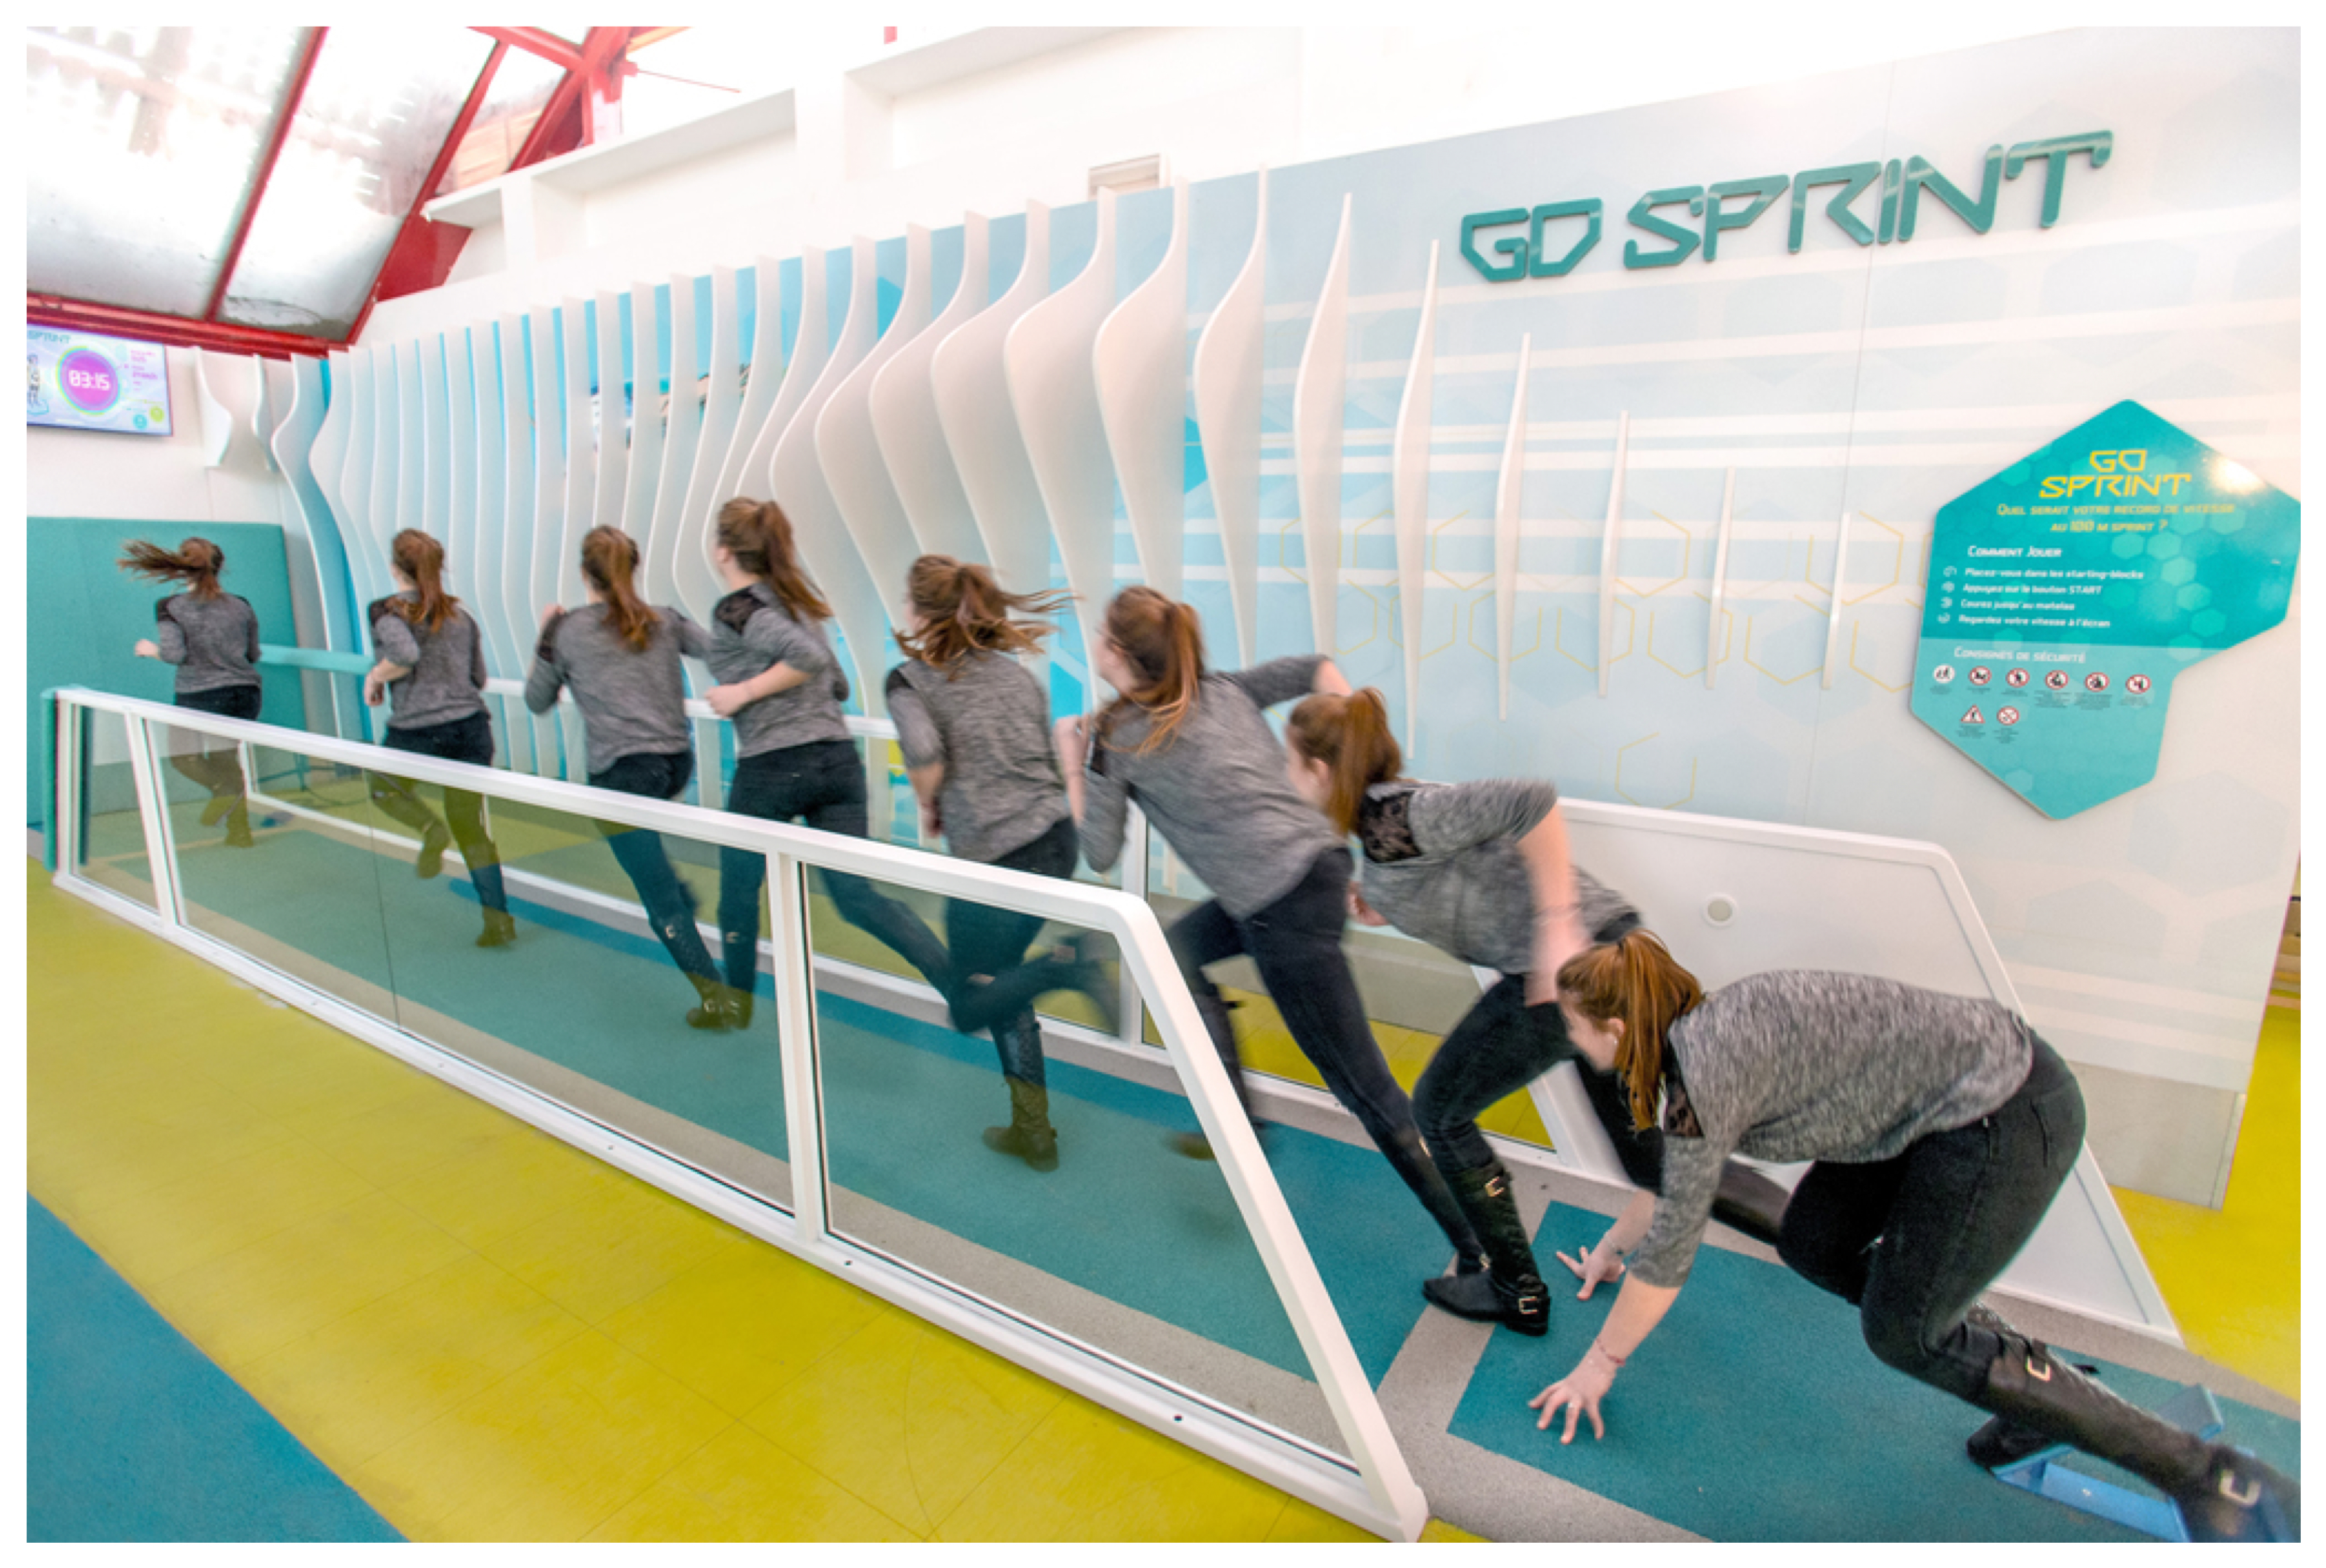
\includegraphics[width=0.9\textwidth]{images/futuroscope.jpg}
        \caption{Credits : Blue Yeti}
    \end{figure}
\end{frame}


\begin{frame}
    \frametitle{Tumbleweed}       
    
    \begin{figure}
    	\centering
    	\includegraphics[width=0.6\textwidth]{images/tumbleweed.jpg}
    	\caption{Credits : Les Baltazars}
    \end{figure}
\end{frame}

\begin{frame}
    \frametitle{Jamoma}       
    
    \begin{figure}
        \centering
        \includegraphics[width=\textwidth]{images/jamoma.jpg}
    \end{figure}
\end{frame}

\begin{frame}
    \frametitle{The software}    
    \begin{figure}
    	\centering
    	\includegraphics[width=\textwidth]{images/iscore.png}
    \end{figure}    
\end{frame}


\begin{frame}
    \frametitle{Contributors, Companies, Agencies involved}
    \begin{figure}[htbp]
    \begin{subfigure}[b]{0.30\textwidth} 
        \centering
        
\begin{tikzpicture}[scale=.05]

\pgfmathsetmacro\bleulabriR{0/255}
\pgfmathsetmacro\bleulabriG{114/255}
\pgfmathsetmacro\bleulabriB{185/255}

\pgfmathsetmacro\vertlabriR{10/255}
\pgfmathsetmacro\vertlabriG{177/255}
\pgfmathsetmacro\vertlabriB{134/255}

\pgfmathsetmacro\rougelabritopR{162/255}
\pgfmathsetmacro\rougelabritopG{47/255}
\pgfmathsetmacro\rougelabritopB{50/255}

\pgfmathsetmacro\rougelabrimiddleR{178/255}
\pgfmathsetmacro\rougelabrimiddleG{117/255}
\pgfmathsetmacro\rougelabrimiddleB{99/255}

\pgfmathsetmacro\rougelabribottomR{230/255}
\pgfmathsetmacro\rougelabribottomG{206/255}
\pgfmathsetmacro\rougelabribottomB{196/255}


\definecolor{bleulabri}{rgb}{\bleulabriR, \bleulabriG, \bleulabriB}
\definecolor{vertlabri}{rgb}{\vertlabriR, \vertlabriG, \vertlabriB}
\definecolor{rougetoplabri}{rgb}{\rougelabritopR, \rougelabritopG,
 \rougelabritopB}
\definecolor{rougemiddlelabri}{rgb}{\rougelabrimiddleR,
 \rougelabrimiddleG, \rougelabrimiddleB}
\definecolor{rougebottomlabri}{rgb}{\rougelabribottomR,
 \rougelabribottomG, \rougelabribottomB}

\def\rectanglepath{-- ++(0cm,38.5cm)-- ++(10cm,0cm)--
 ++(0cm,-30.3cm)-- ++(13cm,0cm)-- ++(-2cm,-8.2cm)-- cycle}


\shade[top color=rougetoplabri!95!black,bottom
 color=rougebottomlabri!15!white!95!black,middle
 color=rougemiddlelabri!90!white!98!black,shading=axis,
shading angle=-135] (19.25, 19.25) circle (6.75cm);

\fill[fill=bleulabri] (0,0) \rectanglepath;
\fill[rotate=180,fill=vertlabri] (-38.5,-38.5) \rectanglepath;

\end{tikzpicture}

        \caption{LaBRI \\ \url{www.labri.fr}}
    \end{subfigure}
    ~
    \begin{subfigure}[b]{0.30\textwidth} 
        \centering
        \includegraphics[scale=0.12]{images/by.png}
        \caption[]{Blue Yeti\\ \url{www.blueyeti.fr}}
    \end{subfigure}
    ~
    \begin{subfigure}[b]{0.30\textwidth} 
        \centering
        \includegraphics[scale=0.15]{images/gmea.png}
        \caption[]{GMEA\\\url{www.gmea.net}}
    \end{subfigure}
    
    
    \begin{subfigure}[b]{0.30\textwidth} 
        \centering
        \includegraphics[scale=0.25]{images/cnam.png}
        \caption[]{CNAM : \\ CEDRIC, ENJMIN\\ \url{cedric.cnam.fr}}
    \end{subfigure}
    ~
    \begin{subfigure}[b]{0.30\textwidth} 
        \centering
        \includegraphics[scale=0.05]{images/ists.jpg}
        \caption[]{ISTS\\ \url{ists-avignon.com}}
    \end{subfigure}
    ~
    \begin{subfigure}[b]{0.30\textwidth} 
        \centering
        \includegraphics[scale=0.23]{images/ensatt.jpg}
        \caption[]{ENSATT\\ \url{ensatt.fr}}
    \end{subfigure}    
\end{figure} 
    
    {\large Artists: Les Baltazars, Renaud Rubiano, Antoine Villeret...}
    
\end{frame}

\setbeamertemplate{frametitle}[default][left]
    \begin{frame}
        \frametitle{What i-score is : }
        \Large
        \begin{itemize}        
        \item<1-> A visual \textbf{programming language} \\ $\rightarrow$ Conditions, loops, structuring, in a timeline\\~\\
        \item<2-> Free software : \textbf{GPL v3 }(UI) \& LGPL v2.1 (Engine)
        \item<2-> Built in \textbf{C++} (Qt, CMake)        
        \item<2-> Available on Linux / OS X / Windows\\ ~\\
        \item<3-> Alpha-quality \DejaSans{☹}
        \end{itemize}
    \end{frame}
    \begin{frame}
        \frametitle{What i-score is not : }
        \Large
        \begin{itemize} [<+->]
            \item PureData (yet)
            \item Ableton Live (yet)       
            \item Bug-free (yet ! \DejaSans{☺})
        \end{itemize}
        \vspace{2em}
        
        \pause[\thebeamerpauses]
        \Huge Does not operate on its own !
        \Large
        \begin{itemize} 
            \item  It's a control center
        \end{itemize}
    \end{frame}
    
    \begin{frame}
    	\centering \Huge Demonstration
    \end{frame}
    
    \begin{frame}
        \frametitle{Inter-operability}
        \Large
        \begin{itemize}
        	\item Compatible environments :\\
	        	 Max/MSP, \textbf{PureData}, Unity3D, \textbf{OpenFrameworks}, \textbf{Processing}, \textbf{Jamoma}, Modul8, Millumin, Quartz Composer, \textbf{Qt}... 
	        \item Anything that communicates over \textbf{OSC}.
	        \item Extensibilty via \textbf{plug-ins}*. \\ {\small *API not stable until v 2.0}
        \end{itemize}
        
    \end{frame}
    
    
    \begin{frame}
        \frametitle{Conditions}
        \begin{figure}
            \centering\psscalebox{0.8}{
            \input{images/cond.tex}}
        \end{figure}    
    \end{frame}
    
    \begin{frame}
        \frametitle{Triggering}
        \begin{figure}
            \centering\psscalebox{0.8}{
                %LaTeX with PSTricks extensions
%%Creator: inkscape 0.91
%%Please note this file requires PSTricks extensions
\psset{xunit=.5pt,yunit=.5pt,runit=.5pt}
\begin{pspicture}(744.09448819,1052.36220472)
{
\newrgbcolor{curcolor}{0.14509805 0.16078432 0.1882353}
\pscustom[linewidth=1,linecolor=curcolor,strokeopacity=0.15686299]
{
\newpath
\moveto(-245.56764,-12.59498528)
\lineto(1005.20236,-12.59498528)
}
}
{
\newrgbcolor{curcolor}{1 0.88235295 0}
\pscustom[linestyle=none,fillstyle=solid,fillcolor=curcolor]
{
\newpath
\moveto(389.38222392,980.01760285)
\lineto(376.69013899,980.01760285)
\lineto(376.69013899,948.48101971)
\lineto(372.03022871,948.48101971)
\lineto(372.03022871,980.01760285)
\lineto(359.33517,980.01760285)
\lineto(359.33517,984.53749472)
\lineto(389.38222392,984.53749472)
\lineto(389.38222392,980.01760285)
}
}
{
\newrgbcolor{curcolor}{1 0.88235295 0}
\pscustom[linestyle=none,fillstyle=solid,fillcolor=curcolor]
{
\newpath
\moveto(383.28003126,969.25256068)
\lineto(374.35869696,958.67572852)
\lineto(365.43736266,969.25256068)
\lineto(383.28003126,969.25256068)
}
}
{
\newrgbcolor{curcolor}{0.27450982 0.27450982 0.27450982}
\pscustom[linestyle=none,fillstyle=solid,fillcolor=curcolor]
{
\newpath
\moveto(373.43236,943.69072472)
\lineto(375.43236,943.69072472)
\lineto(375.43236,673.69072472)
\lineto(373.43236,673.69072472)
\closepath
}
}
{
\newrgbcolor{curcolor}{0.48627451 0.48627451 0.48627451}
\pscustom[linestyle=none,fillstyle=solid,fillcolor=curcolor]
{
\newpath
\moveto(373.13236005,943.69072472)
\lineto(375.73235995,943.69072472)
\lineto(375.73235995,673.69072472)
\lineto(373.13236005,673.69072472)
\closepath
}
}
{
\newrgbcolor{curcolor}{0.01176471 0.7647059 0.86666667}
\pscustom[linewidth=2.28296474,linecolor=curcolor]
{
\newpath
\moveto(111.98631,943.69072472)
\lineto(204.06370449,943.69072472)
}
}
{
\newrgbcolor{curcolor}{0.01176471 0.7647059 0.86666667}
\pscustom[linewidth=3,linecolor=curcolor,linestyle=dashed,dash=6 18]
{
\newpath
\moveto(203.43236,943.69072472)
\lineto(440.43236,943.69072472)
}
}
{
\newrgbcolor{curcolor}{0.01176471 0.7647059 0.86666667}
\pscustom[linewidth=2,linecolor=curcolor]
{
\newpath
\moveto(203.43236,953.69072472)
\curveto(197.90951,953.69072472)(193.43236,949.21357472)(193.43236,943.69072472)
\curveto(193.43236,938.16787472)(197.90951,933.69072472)(203.43236,933.69072472)
\lineto(203.43236,953.69072472)
}
}
{
\newrgbcolor{curcolor}{0.01176471 0.7647059 0.86666667}
\pscustom[linewidth=2,linecolor=curcolor]
{
\newpath
\moveto(440.43236,933.69072472)
\curveto(445.95521,933.69072472)(450.43236,938.16787472)(450.43236,943.69072472)
\curveto(450.43236,949.21357472)(445.95521,953.69072472)(440.43236,953.69072472)
\lineto(440.43236,933.69072472)
}
}
{
\newrgbcolor{curcolor}{0.01176471 0.7647059 0.86666667}
\pscustom[linewidth=3,linecolor=curcolor]
{
\newpath
\moveto(44.43236,803.69072472)
\lineto(308.43236,803.69072472)
}
}
{
\newrgbcolor{curcolor}{0.01176471 0.7647059 0.86666667}
\pscustom[linewidth=3,linecolor=curcolor,linestyle=dashed,dash=6 18]
{
\newpath
\moveto(308.43236,803.69072472)
\lineto(525.43236,803.69072472)
}
}
{
\newrgbcolor{curcolor}{0.01176471 0.7647059 0.86666667}
\pscustom[linewidth=2,linecolor=curcolor]
{
\newpath
\moveto(308.43236,813.69072472)
\curveto(302.90951,813.69072472)(298.43236,809.21357472)(298.43236,803.69072472)
\curveto(298.43236,798.16787472)(302.90951,793.69072472)(308.43236,793.69072472)
\lineto(308.43236,813.69072472)
}
}
{
\newrgbcolor{curcolor}{0.01176471 0.7647059 0.86666667}
\pscustom[linewidth=2,linecolor=curcolor]
{
\newpath
\moveto(525.43236,793.69072472)
\curveto(530.95521,793.69072472)(535.43236,798.16787472)(535.43236,803.69072472)
\curveto(535.43236,809.21357472)(530.95521,813.69072472)(525.43236,813.69072472)
\lineto(525.43236,793.69072472)
}
}
{
\newrgbcolor{curcolor}{0.01176471 0.7647059 0.86666667}
\pscustom[linewidth=3,linecolor=curcolor]
{
\newpath
\moveto(374.43236,673.69072472)
\lineto(563.43236,673.69072472)
}
}
{
\newrgbcolor{curcolor}{0.14509805 0.16078432 0.1882353}
\pscustom[linestyle=none,fillstyle=solid,fillcolor=curcolor]
{
\newpath
\moveto(115.07197,943.69072472)
\curveto(115.07197,939.82473148)(111.93796325,936.69072472)(108.07197,936.69072472)
\curveto(104.20597675,936.69072472)(101.07197,939.82473148)(101.07197,943.69072472)
\curveto(101.07197,947.55671797)(104.20597675,950.69072472)(108.07197,950.69072472)
\curveto(111.93796325,950.69072472)(115.07197,947.55671797)(115.07197,943.69072472)
\closepath
}
}
{
\newrgbcolor{curcolor}{0.627451 0.627451 0.64313728}
\pscustom[linewidth=2,linecolor=curcolor]
{
\newpath
\moveto(115.07197,943.69072472)
\curveto(115.07197,939.82473148)(111.93796325,936.69072472)(108.07197,936.69072472)
\curveto(104.20597675,936.69072472)(101.07197,939.82473148)(101.07197,943.69072472)
\curveto(101.07197,947.55671797)(104.20597675,950.69072472)(108.07197,950.69072472)
\curveto(111.93796325,950.69072472)(115.07197,947.55671797)(115.07197,943.69072472)
\closepath
}
}
{
\newrgbcolor{curcolor}{0.14509805 0.16078432 0.1882353}
\pscustom[linestyle=none,fillstyle=solid,fillcolor=curcolor]
{
\newpath
\moveto(381.43236,943.69072472)
\curveto(381.43236,939.82473148)(378.29835325,936.69072472)(374.43236,936.69072472)
\curveto(370.56636675,936.69072472)(367.43236,939.82473148)(367.43236,943.69072472)
\curveto(367.43236,947.55671797)(370.56636675,950.69072472)(374.43236,950.69072472)
\curveto(378.29835325,950.69072472)(381.43236,947.55671797)(381.43236,943.69072472)
\closepath
}
}
{
\newrgbcolor{curcolor}{0.627451 0.627451 0.64313728}
\pscustom[linewidth=2,linecolor=curcolor]
{
\newpath
\moveto(381.43236,943.69072472)
\curveto(381.43236,939.82473148)(378.29835325,936.69072472)(374.43236,936.69072472)
\curveto(370.56636675,936.69072472)(367.43236,939.82473148)(367.43236,943.69072472)
\curveto(367.43236,947.55671797)(370.56636675,950.69072472)(374.43236,950.69072472)
\curveto(378.29835325,950.69072472)(381.43236,947.55671797)(381.43236,943.69072472)
\closepath
}
}
{
\newrgbcolor{curcolor}{0.14509805 0.16078432 0.1882353}
\pscustom[linestyle=none,fillstyle=solid,fillcolor=curcolor]
{
\newpath
\moveto(381.43236,803.69072472)
\curveto(381.43236,799.82473148)(378.29835325,796.69072472)(374.43236,796.69072472)
\curveto(370.56636675,796.69072472)(367.43236,799.82473148)(367.43236,803.69072472)
\curveto(367.43236,807.55671797)(370.56636675,810.69072472)(374.43236,810.69072472)
\curveto(378.29835325,810.69072472)(381.43236,807.55671797)(381.43236,803.69072472)
\closepath
}
}
{
\newrgbcolor{curcolor}{0.627451 0.627451 0.64313728}
\pscustom[linewidth=2,linecolor=curcolor]
{
\newpath
\moveto(381.43236,803.69072472)
\curveto(381.43236,799.82473148)(378.29835325,796.69072472)(374.43236,796.69072472)
\curveto(370.56636675,796.69072472)(367.43236,799.82473148)(367.43236,803.69072472)
\curveto(367.43236,807.55671797)(370.56636675,810.69072472)(374.43236,810.69072472)
\curveto(378.29835325,810.69072472)(381.43236,807.55671797)(381.43236,803.69072472)
\closepath
}
}
{
\newrgbcolor{curcolor}{0.14509805 0.16078432 0.1882353}
\pscustom[linestyle=none,fillstyle=solid,fillcolor=curcolor]
{
\newpath
\moveto(51.43236,803.69072472)
\curveto(51.43236,799.82473148)(48.29835325,796.69072472)(44.43236,796.69072472)
\curveto(40.56636675,796.69072472)(37.43236,799.82473148)(37.43236,803.69072472)
\curveto(37.43236,807.55671797)(40.56636675,810.69072472)(44.43236,810.69072472)
\curveto(48.29835325,810.69072472)(51.43236,807.55671797)(51.43236,803.69072472)
\closepath
}
}
{
\newrgbcolor{curcolor}{0.627451 0.627451 0.64313728}
\pscustom[linewidth=2,linecolor=curcolor]
{
\newpath
\moveto(51.43236,803.69072472)
\curveto(51.43236,799.82473148)(48.29835325,796.69072472)(44.43236,796.69072472)
\curveto(40.56636675,796.69072472)(37.43236,799.82473148)(37.43236,803.69072472)
\curveto(37.43236,807.55671797)(40.56636675,810.69072472)(44.43236,810.69072472)
\curveto(48.29835325,810.69072472)(51.43236,807.55671797)(51.43236,803.69072472)
\closepath
}
}
{
\newrgbcolor{curcolor}{0.14509805 0.16078432 0.1882353}
\pscustom[linestyle=none,fillstyle=solid,fillcolor=curcolor]
{
\newpath
\moveto(381.43236,673.69072472)
\curveto(381.43236,669.82473148)(378.29835325,666.69072472)(374.43236,666.69072472)
\curveto(370.56636675,666.69072472)(367.43236,669.82473148)(367.43236,673.69072472)
\curveto(367.43236,677.55671797)(370.56636675,680.69072472)(374.43236,680.69072472)
\curveto(378.29835325,680.69072472)(381.43236,677.55671797)(381.43236,673.69072472)
\closepath
}
}
{
\newrgbcolor{curcolor}{0.627451 0.627451 0.64313728}
\pscustom[linewidth=2,linecolor=curcolor]
{
\newpath
\moveto(381.43236,673.69072472)
\curveto(381.43236,669.82473148)(378.29835325,666.69072472)(374.43236,666.69072472)
\curveto(370.56636675,666.69072472)(367.43236,669.82473148)(367.43236,673.69072472)
\curveto(367.43236,677.55671797)(370.56636675,680.69072472)(374.43236,680.69072472)
\curveto(378.29835325,680.69072472)(381.43236,677.55671797)(381.43236,673.69072472)
\closepath
}
}
{
\newrgbcolor{curcolor}{0.14509805 0.16078432 0.1882353}
\pscustom[linestyle=none,fillstyle=solid,fillcolor=curcolor]
{
\newpath
\moveto(570.43236,673.69072472)
\curveto(570.43236,669.82473148)(567.29835325,666.69072472)(563.43236,666.69072472)
\curveto(559.56636675,666.69072472)(556.43236,669.82473148)(556.43236,673.69072472)
\curveto(556.43236,677.55671797)(559.56636675,680.69072472)(563.43236,680.69072472)
\curveto(567.29835325,680.69072472)(570.43236,677.55671797)(570.43236,673.69072472)
\closepath
}
}
{
\newrgbcolor{curcolor}{0.627451 0.627451 0.64313728}
\pscustom[linewidth=2,linecolor=curcolor]
{
\newpath
\moveto(570.43236,673.69072472)
\curveto(570.43236,669.82473148)(567.29835325,666.69072472)(563.43236,666.69072472)
\curveto(559.56636675,666.69072472)(556.43236,669.82473148)(556.43236,673.69072472)
\curveto(556.43236,677.55671797)(559.56636675,680.69072472)(563.43236,680.69072472)
\curveto(567.29835325,680.69072472)(570.43236,677.55671797)(570.43236,673.69072472)
\closepath
}
}
{
\newrgbcolor{curcolor}{0 0 0}
\pscustom[linestyle=none,fillstyle=solid,fillcolor=curcolor]
{
\newpath
\moveto(112.18151771,1001.53248054)
\lineto(107.58151771,1016.28248054)
\lineto(105.25651771,1016.28248054)
\lineto(111.00651771,999.05748054)
\lineto(113.25651771,999.05748054)
\lineto(119.00651771,1016.28248054)
\lineto(116.83151771,1016.28248054)
\lineto(112.18151771,1001.53248054)
\closepath
}
}
{
\newrgbcolor{curcolor}{0 0 0}
\pscustom[linestyle=none,fillstyle=solid,fillcolor=curcolor]
{
\newpath
\moveto(127.12175209,1018.38248054)
\curveto(126.22175209,1018.38248054)(125.62175209,1017.75748054)(125.62175209,1016.90748054)
\curveto(125.62175209,1016.05748054)(126.22175209,1015.43248054)(127.12175209,1015.43248054)
\curveto(128.04675209,1015.43248054)(128.67175209,1016.05748054)(128.67175209,1016.90748054)
\curveto(128.67175209,1017.75748054)(128.04675209,1018.38248054)(127.12175209,1018.38248054)
\closepath
\moveto(128.79675209,1012.23248054)
\lineto(122.77175209,1012.23248054)
\lineto(122.77175209,1010.55748054)
\lineto(126.69675209,1010.55748054)
\lineto(126.69675209,1000.73248054)
\lineto(122.64675209,1000.73248054)
\lineto(122.64675209,999.05748054)
\lineto(132.49675209,999.05748054)
\lineto(132.49675209,1000.73248054)
\lineto(128.79675209,1000.73248054)
\lineto(128.79675209,1012.23248054)
\closepath
}
}
{
\newrgbcolor{curcolor}{0 0 0}
\pscustom[linestyle=none,fillstyle=solid,fillcolor=curcolor]
{
\newpath
\moveto(145.01198646,1017.78248054)
\lineto(145.01198646,1010.93248054)
\curveto(144.11198646,1011.95748054)(142.98698646,1012.50748054)(141.46198646,1012.50748054)
\curveto(138.23698646,1012.50748054)(136.31198646,1009.58248054)(136.31198646,1005.63248054)
\curveto(136.31198646,1001.53248054)(137.88698646,998.78248054)(141.33698646,998.78248054)
\curveto(142.76198646,998.78248054)(144.08698646,999.40748054)(145.06198646,1000.78248054)
\lineto(145.26198646,999.05748054)
\lineto(147.11198646,999.05748054)
\lineto(147.11198646,1017.53248054)
\lineto(145.01198646,1017.78248054)
\closepath
\moveto(142.01198646,1010.80748054)
\curveto(143.23698646,1010.80748054)(144.28698646,1010.18248054)(145.01198646,1009.10748054)
\lineto(145.01198646,1002.55748054)
\curveto(144.28698646,1001.45748054)(143.26198646,1000.45748054)(141.76198646,1000.45748054)
\curveto(139.68698646,1000.45748054)(138.58698646,1002.20748054)(138.58698646,1005.63248054)
\curveto(138.58698646,1009.10748054)(139.83698646,1010.80748054)(142.01198646,1010.80748054)
\closepath
}
}
{
\newrgbcolor{curcolor}{0 0 0}
\pscustom[linestyle=none,fillstyle=solid,fillcolor=curcolor]
{
\newpath
\moveto(153.77722084,1004.90748054)
\lineto(162.62722084,1004.90748054)
\curveto(162.65222084,1005.18248054)(162.67722084,1005.58248054)(162.67722084,1006.03248054)
\curveto(162.67722084,1010.03248054)(160.62722084,1012.50748054)(157.30222084,1012.50748054)
\curveto(153.80222084,1012.50748054)(151.57722084,1009.60748054)(151.57722084,1005.63248054)
\curveto(151.57722084,1001.53248054)(153.75222084,998.78248054)(157.60222084,998.78248054)
\curveto(159.22722084,998.78248054)(160.87722084,999.35748054)(162.10222084,1000.30748054)
\lineto(161.12722084,1001.70748054)
\curveto(159.95222084,1000.93248054)(158.95222084,1000.53248054)(157.60222084,1000.53248054)
\curveto(155.57722084,1000.53248054)(153.87722084,1001.85748054)(153.77722084,1004.90748054)
\closepath
\moveto(157.32722084,1010.78248054)
\curveto(159.32722084,1010.78248054)(160.57722084,1009.33248054)(160.62722084,1006.50748054)
\lineto(153.77722084,1006.50748054)
\curveto(153.95222084,1009.40748054)(155.37722084,1010.78248054)(157.32722084,1010.78248054)
\closepath
}
}
{
\newrgbcolor{curcolor}{0 0 0}
\pscustom[linestyle=none,fillstyle=solid,fillcolor=curcolor]
{
\newpath
\moveto(172.11745521,1012.50748054)
\curveto(168.41745521,1012.50748054)(166.41745521,1009.68248054)(166.41745521,1005.63248054)
\curveto(166.41745521,1001.48248054)(168.39245521,998.78248054)(172.09245521,998.78248054)
\curveto(175.76745521,998.78248054)(177.76745521,1001.60748054)(177.76745521,1005.65748054)
\curveto(177.76745521,1009.80748054)(175.81745521,1012.50748054)(172.11745521,1012.50748054)
\closepath
\moveto(172.11745521,1010.78248054)
\curveto(174.36745521,1010.78248054)(175.49245521,1009.13248054)(175.49245521,1005.65748054)
\curveto(175.49245521,1002.13248054)(174.36745521,1000.50748054)(172.09245521,1000.50748054)
\curveto(169.81745521,1000.50748054)(168.69245521,1002.13248054)(168.69245521,1005.63248054)
\curveto(168.69245521,1009.13248054)(169.84245521,1010.78248054)(172.11745521,1010.78248054)
\closepath
}
}
{
\newrgbcolor{curcolor}{0 0 0}
\pscustom[linestyle=none,fillstyle=solid,fillcolor=curcolor]
{
\newpath
\moveto(185.05768959,1009.83248054)
\curveto(185.05768959,1008.70748054)(185.90768959,1007.78248054)(187.05768959,1007.78248054)
\curveto(188.23268959,1007.78248054)(189.08268959,1008.70748054)(189.08268959,1009.83248054)
\curveto(189.08268959,1010.93248054)(188.23268959,1011.83248054)(187.05768959,1011.83248054)
\curveto(185.90768959,1011.83248054)(185.05768959,1010.93248054)(185.05768959,1009.83248054)
\closepath
\moveto(185.05768959,1000.80748054)
\curveto(185.05768959,999.65748054)(185.90768959,998.78248054)(187.05768959,998.78248054)
\curveto(188.23268959,998.78248054)(189.08268959,999.65748054)(189.08268959,1000.80748054)
\curveto(189.08268959,1001.90748054)(188.23268959,1002.83248054)(187.05768959,1002.83248054)
\curveto(185.90768959,1002.83248054)(185.05768959,1001.90748054)(185.05768959,1000.80748054)
\closepath
}
}
{
\newrgbcolor{curcolor}{0 0 0}
\pscustom[linestyle=none,fillstyle=solid,fillcolor=curcolor]
{
\newpath
\moveto(197.59792396,996.48248054)
\lineto(208.24792396,1018.48248054)
\lineto(206.57292396,1019.28248054)
\lineto(195.89792396,997.23248054)
\lineto(197.59792396,996.48248054)
\closepath
}
}
{
\newrgbcolor{curcolor}{0 0 0}
\pscustom[linestyle=none,fillstyle=solid,fillcolor=curcolor]
{
\newpath
\moveto(217.96315834,1012.50748054)
\curveto(216.38815834,1012.50748054)(214.98815834,1011.73248054)(214.03815834,1010.38248054)
\lineto(213.86315834,1012.23248054)
\lineto(212.06315834,1012.23248054)
\lineto(212.06315834,993.75748054)
\lineto(214.16315834,994.00748054)
\lineto(214.16315834,1000.28248054)
\curveto(215.06315834,999.28248054)(216.21315834,998.78248054)(217.66315834,998.78248054)
\curveto(221.08815834,998.78248054)(222.73815834,1001.65748054)(222.73815834,1005.65748054)
\curveto(222.73815834,1009.78248054)(221.46315834,1012.50748054)(217.96315834,1012.50748054)
\closepath
\moveto(217.46315834,1010.80748054)
\curveto(219.53815834,1010.80748054)(220.46315834,1009.08248054)(220.46315834,1005.65748054)
\curveto(220.46315834,1002.15748054)(219.36315834,1000.53248054)(217.18815834,1000.53248054)
\curveto(215.93815834,1000.53248054)(214.86315834,1001.15748054)(214.16315834,1002.18248054)
\lineto(214.16315834,1008.70748054)
\curveto(214.88815834,1009.75748054)(216.01315834,1010.80748054)(217.46315834,1010.80748054)
\closepath
}
}
{
\newrgbcolor{curcolor}{0 0 0}
\pscustom[linestyle=none,fillstyle=solid,fillcolor=curcolor]
{
\newpath
\moveto(232.07839271,1012.50748054)
\curveto(228.37839271,1012.50748054)(226.37839271,1009.68248054)(226.37839271,1005.63248054)
\curveto(226.37839271,1001.48248054)(228.35339271,998.78248054)(232.05339271,998.78248054)
\curveto(235.72839271,998.78248054)(237.72839271,1001.60748054)(237.72839271,1005.65748054)
\curveto(237.72839271,1009.80748054)(235.77839271,1012.50748054)(232.07839271,1012.50748054)
\closepath
\moveto(232.07839271,1010.78248054)
\curveto(234.32839271,1010.78248054)(235.45339271,1009.13248054)(235.45339271,1005.65748054)
\curveto(235.45339271,1002.13248054)(234.32839271,1000.50748054)(232.05339271,1000.50748054)
\curveto(229.77839271,1000.50748054)(228.65339271,1002.13248054)(228.65339271,1005.63248054)
\curveto(228.65339271,1009.13248054)(229.80339271,1010.78248054)(232.07839271,1010.78248054)
\closepath
}
}
{
\newrgbcolor{curcolor}{0 0 0}
\pscustom[linestyle=none,fillstyle=solid,fillcolor=curcolor]
{
\newpath
\moveto(242.04362709,999.05748054)
\lineto(244.14362709,999.05748054)
\lineto(244.14362709,1008.63248054)
\curveto(244.84362709,1009.68248054)(246.16862709,1010.83248054)(247.71862709,1010.83248054)
\curveto(249.69362709,1010.83248054)(249.96862709,1009.75748054)(249.96862709,1007.05748054)
\lineto(249.96862709,999.05748054)
\lineto(252.06862709,999.05748054)
\lineto(252.06862709,1008.60748054)
\curveto(252.06862709,1011.05748054)(250.94362709,1012.50748054)(248.36862709,1012.50748054)
\curveto(246.81862709,1012.50748054)(245.06862709,1011.73248054)(244.01862709,1010.38248054)
\lineto(243.84362709,1012.23248054)
\lineto(242.04362709,1012.23248054)
\lineto(242.04362709,999.05748054)
\closepath
}
}
{
\newrgbcolor{curcolor}{0 0 0}
\pscustom[linestyle=none,fillstyle=solid,fillcolor=curcolor]
{
\newpath
\moveto(267.98386146,1012.23248054)
\lineto(265.80886146,1012.23248054)
\lineto(262.08386146,1000.65748054)
\lineto(258.30886146,1012.23248054)
\lineto(256.08386146,1012.23248054)
\lineto(260.65886146,999.05748054)
\lineto(261.35886146,999.05748054)
\curveto(260.68386146,997.03248054)(259.88386146,995.90748054)(257.18386146,995.43248054)
\lineto(257.48386146,993.75748054)
\curveto(260.98386146,994.13248054)(262.45886146,996.28248054)(263.38386146,998.98248054)
\lineto(267.98386146,1012.23248054)
\closepath
}
}
{
\newrgbcolor{curcolor}{0 0 0}
\pscustom[linestyle=none,fillstyle=solid,fillcolor=curcolor]
{
\newpath
\moveto(272.54909584,996.48248054)
\lineto(283.19909584,1018.48248054)
\lineto(281.52409584,1019.28248054)
\lineto(270.84909584,997.23248054)
\lineto(272.54909584,996.48248054)
\closepath
}
}
{
\newrgbcolor{curcolor}{0 0 0}
\pscustom[linestyle=none,fillstyle=solid,fillcolor=curcolor]
{
\newpath
\moveto(289.11433021,1010.50748054)
\lineto(289.11433021,1017.78248054)
\lineto(287.01433021,1017.53248054)
\lineto(287.01433021,999.05748054)
\lineto(288.86433021,999.05748054)
\lineto(289.01433021,1000.43248054)
\curveto(289.91433021,999.28248054)(291.08933021,998.78248054)(292.58933021,998.78248054)
\curveto(295.98933021,998.78248054)(297.81433021,1001.65748054)(297.81433021,1005.65748054)
\curveto(297.81433021,1009.78248054)(296.38933021,1012.50748054)(292.88933021,1012.50748054)
\curveto(291.36433021,1012.50748054)(290.08933021,1011.78248054)(289.11433021,1010.50748054)
\closepath
\moveto(292.11433021,1000.48248054)
\curveto(290.88933021,1000.48248054)(289.81433021,1001.10748054)(289.11433021,1002.18248054)
\lineto(289.11433021,1008.70748054)
\curveto(289.83933021,1009.75748054)(290.96433021,1010.80748054)(292.41433021,1010.80748054)
\curveto(294.46433021,1010.80748054)(295.53933021,1009.08248054)(295.53933021,1005.65748054)
\curveto(295.53933021,1002.15748054)(294.28933021,1000.48248054)(292.11433021,1000.48248054)
\closepath
}
}
{
\newrgbcolor{curcolor}{0 0 0}
\pscustom[linestyle=none,fillstyle=solid,fillcolor=curcolor]
{
\newpath
\moveto(303.67956459,1004.90748054)
\lineto(312.52956459,1004.90748054)
\curveto(312.55456459,1005.18248054)(312.57956459,1005.58248054)(312.57956459,1006.03248054)
\curveto(312.57956459,1010.03248054)(310.52956459,1012.50748054)(307.20456459,1012.50748054)
\curveto(303.70456459,1012.50748054)(301.47956459,1009.60748054)(301.47956459,1005.63248054)
\curveto(301.47956459,1001.53248054)(303.65456459,998.78248054)(307.50456459,998.78248054)
\curveto(309.12956459,998.78248054)(310.77956459,999.35748054)(312.00456459,1000.30748054)
\lineto(311.02956459,1001.70748054)
\curveto(309.85456459,1000.93248054)(308.85456459,1000.53248054)(307.50456459,1000.53248054)
\curveto(305.47956459,1000.53248054)(303.77956459,1001.85748054)(303.67956459,1004.90748054)
\closepath
\moveto(307.22956459,1010.78248054)
\curveto(309.22956459,1010.78248054)(310.47956459,1009.33248054)(310.52956459,1006.50748054)
\lineto(303.67956459,1006.50748054)
\curveto(303.85456459,1009.40748054)(305.27956459,1010.78248054)(307.22956459,1010.78248054)
\closepath
}
}
{
\newrgbcolor{curcolor}{0 0 0}
\pscustom[linestyle=none,fillstyle=solid,fillcolor=curcolor]
{
\newpath
\moveto(321.49479896,1000.50748054)
\curveto(319.94479896,1000.50748054)(318.54479896,1001.08248054)(317.51979896,1001.93248054)
\lineto(316.34479896,1000.55748054)
\curveto(317.46979896,999.58248054)(319.09479896,998.78248054)(321.49479896,998.78248054)
\curveto(324.29479896,998.78248054)(327.01979896,999.88248054)(327.01979896,1002.70748054)
\curveto(327.01979896,1005.15748054)(325.31979896,1006.05748054)(322.74479896,1006.75748054)
\curveto(320.09479896,1007.48248054)(319.26979896,1007.88248054)(319.26979896,1009.08248054)
\curveto(319.26979896,1010.08248054)(320.01979896,1010.80748054)(322.11979896,1010.80748054)
\curveto(323.81979896,1010.80748054)(324.94479896,1010.28248054)(325.91979896,1009.60748054)
\lineto(326.86979896,1011.05748054)
\curveto(325.74479896,1011.85748054)(324.19479896,1012.50748054)(322.06979896,1012.50748054)
\curveto(319.09479896,1012.50748054)(317.06979896,1011.10748054)(317.06979896,1008.90748054)
\curveto(317.06979896,1006.60748054)(318.84479896,1005.78248054)(321.56979896,1005.10748054)
\curveto(324.36979896,1004.40748054)(324.74479896,1003.78248054)(324.74479896,1002.60748054)
\curveto(324.74479896,1001.33248054)(323.51979896,1000.50748054)(321.49479896,1000.50748054)
\closepath
}
}
{
\newrgbcolor{curcolor}{0 0 0}
\pscustom[linestyle=none,fillstyle=solid,fillcolor=curcolor]
{
\newpath
\moveto(342.46003334,999.73248054)
\lineto(341.63503334,1001.15748054)
\curveto(340.93503334,1000.78248054)(340.08503334,1000.53248054)(339.11003334,1000.53248054)
\curveto(337.31003334,1000.53248054)(336.58503334,1001.30748054)(336.58503334,1002.75748054)
\lineto(336.58503334,1010.58248054)
\lineto(340.88503334,1010.58248054)
\lineto(341.16003334,1012.23248054)
\lineto(336.58503334,1012.23248054)
\lineto(336.58503334,1015.45748054)
\lineto(334.48503334,1015.20748054)
\lineto(334.48503334,1012.23248054)
\lineto(331.46003334,1012.23248054)
\lineto(331.46003334,1010.58248054)
\lineto(334.48503334,1010.58248054)
\lineto(334.48503334,1002.73248054)
\curveto(334.48503334,1000.43248054)(336.08503334,998.78248054)(338.91003334,998.78248054)
\curveto(340.16003334,998.78248054)(341.53503334,999.13248054)(342.46003334,999.73248054)
\closepath
}
}
{
\newrgbcolor{curcolor}{0 0 0}
\pscustom[linestyle=none,fillstyle=solid,fillcolor=curcolor]
{
\newpath
\moveto(386.80573646,1010.10748054)
\lineto(362.10573646,1010.10748054)
\lineto(362.10573646,1008.30748054)
\lineto(386.80573646,1008.30748054)
\lineto(386.80573646,1010.10748054)
\closepath
\moveto(386.80573646,1005.35748054)
\lineto(362.10573646,1005.35748054)
\lineto(362.10573646,1003.55748054)
\lineto(386.80573646,1003.55748054)
\lineto(386.80573646,1005.35748054)
\closepath
}
}
{
\newrgbcolor{curcolor}{0 0 0}
\pscustom[linestyle=none,fillstyle=solid,fillcolor=curcolor]
{
\newpath
\moveto(408.91120521,1011.03248054)
\lineto(410.76120521,1011.03248054)
\lineto(411.16120521,1017.53248054)
\lineto(408.53620521,1017.53248054)
\lineto(408.91120521,1011.03248054)
\closepath
\moveto(413.11120521,1011.03248054)
\lineto(414.96120521,1011.03248054)
\lineto(415.33620521,1017.53248054)
\lineto(412.71120521,1017.53248054)
\lineto(413.11120521,1011.03248054)
\closepath
}
}
{
\newrgbcolor{curcolor}{0 0 0}
\pscustom[linestyle=none,fillstyle=solid,fillcolor=curcolor]
{
\newpath
\moveto(425.05143959,1014.48248054)
\lineto(432.77643959,1014.48248054)
\lineto(433.02643959,1016.28248054)
\lineto(422.87643959,1016.28248054)
\lineto(422.87643959,999.05748054)
\lineto(425.05143959,999.05748054)
\lineto(425.05143959,1006.70748054)
\lineto(431.80143959,1006.70748054)
\lineto(431.80143959,1008.45748054)
\lineto(425.05143959,1008.45748054)
\lineto(425.05143959,1014.48248054)
\closepath
}
}
{
\newrgbcolor{curcolor}{0 0 0}
\pscustom[linestyle=none,fillstyle=solid,fillcolor=curcolor]
{
\newpath
\moveto(442.06667396,1017.53248054)
\lineto(435.91667396,1017.53248054)
\lineto(435.91667396,1015.85748054)
\lineto(439.96667396,1015.85748054)
\lineto(439.96667396,1002.40748054)
\curveto(439.96667396,1000.13248054)(441.54167396,998.78248054)(443.86667396,998.78248054)
\curveto(445.21667396,998.78248054)(446.29167396,999.08248054)(446.99167396,999.45748054)
\lineto(446.44167396,1000.98248054)
\curveto(445.71667396,1000.70748054)(445.01667396,1000.53248054)(444.24167396,1000.53248054)
\curveto(442.96667396,1000.53248054)(442.06667396,1001.00748054)(442.06667396,1002.30748054)
\lineto(442.06667396,1017.53248054)
\closepath
}
}
{
\newrgbcolor{curcolor}{0 0 0}
\pscustom[linestyle=none,fillstyle=solid,fillcolor=curcolor]
{
\newpath
\moveto(454.00690834,1012.23248054)
\lineto(451.90690834,1012.23248054)
\lineto(451.90690834,1002.65748054)
\curveto(451.90690834,1000.20748054)(453.15690834,998.78248054)(455.70690834,998.78248054)
\curveto(457.25690834,998.78248054)(458.88190834,999.50748054)(459.93190834,1000.83248054)
\lineto(460.10690834,999.05748054)
\lineto(461.90690834,999.05748054)
\lineto(461.90690834,1012.23248054)
\lineto(459.80690834,1012.23248054)
\lineto(459.80690834,1002.53248054)
\curveto(459.08190834,1001.40748054)(457.68190834,1000.43248054)(456.23190834,1000.43248054)
\curveto(454.70690834,1000.43248054)(454.00690834,1001.18248054)(454.00690834,1002.88248054)
\lineto(454.00690834,1012.23248054)
\closepath
}
}
{
\newrgbcolor{curcolor}{0 0 0}
\pscustom[linestyle=none,fillstyle=solid,fillcolor=curcolor]
{
\newpath
\moveto(477.37214271,999.73248054)
\lineto(476.54714271,1001.15748054)
\curveto(475.84714271,1000.78248054)(474.99714271,1000.53248054)(474.02214271,1000.53248054)
\curveto(472.22214271,1000.53248054)(471.49714271,1001.30748054)(471.49714271,1002.75748054)
\lineto(471.49714271,1010.58248054)
\lineto(475.79714271,1010.58248054)
\lineto(476.07214271,1012.23248054)
\lineto(471.49714271,1012.23248054)
\lineto(471.49714271,1015.45748054)
\lineto(469.39714271,1015.20748054)
\lineto(469.39714271,1012.23248054)
\lineto(466.37214271,1012.23248054)
\lineto(466.37214271,1010.58248054)
\lineto(469.39714271,1010.58248054)
\lineto(469.39714271,1002.73248054)
\curveto(469.39714271,1000.43248054)(470.99714271,998.78248054)(473.82214271,998.78248054)
\curveto(475.07214271,998.78248054)(476.44714271,999.13248054)(477.37214271,999.73248054)
\closepath
}
}
{
\newrgbcolor{curcolor}{0 0 0}
\pscustom[linestyle=none,fillstyle=solid,fillcolor=curcolor]
{
\newpath
\moveto(492.36237709,999.73248054)
\lineto(491.53737709,1001.15748054)
\curveto(490.83737709,1000.78248054)(489.98737709,1000.53248054)(489.01237709,1000.53248054)
\curveto(487.21237709,1000.53248054)(486.48737709,1001.30748054)(486.48737709,1002.75748054)
\lineto(486.48737709,1010.58248054)
\lineto(490.78737709,1010.58248054)
\lineto(491.06237709,1012.23248054)
\lineto(486.48737709,1012.23248054)
\lineto(486.48737709,1015.45748054)
\lineto(484.38737709,1015.20748054)
\lineto(484.38737709,1012.23248054)
\lineto(481.36237709,1012.23248054)
\lineto(481.36237709,1010.58248054)
\lineto(484.38737709,1010.58248054)
\lineto(484.38737709,1002.73248054)
\curveto(484.38737709,1000.43248054)(485.98737709,998.78248054)(488.81237709,998.78248054)
\curveto(490.06237709,998.78248054)(491.43737709,999.13248054)(492.36237709,999.73248054)
\closepath
}
}
{
\newrgbcolor{curcolor}{0 0 0}
\pscustom[linestyle=none,fillstyle=solid,fillcolor=curcolor]
{
\newpath
\moveto(498.55261146,1004.90748054)
\lineto(507.40261146,1004.90748054)
\curveto(507.42761146,1005.18248054)(507.45261146,1005.58248054)(507.45261146,1006.03248054)
\curveto(507.45261146,1010.03248054)(505.40261146,1012.50748054)(502.07761146,1012.50748054)
\curveto(498.57761146,1012.50748054)(496.35261146,1009.60748054)(496.35261146,1005.63248054)
\curveto(496.35261146,1001.53248054)(498.52761146,998.78248054)(502.37761146,998.78248054)
\curveto(504.00261146,998.78248054)(505.65261146,999.35748054)(506.87761146,1000.30748054)
\lineto(505.90261146,1001.70748054)
\curveto(504.72761146,1000.93248054)(503.72761146,1000.53248054)(502.37761146,1000.53248054)
\curveto(500.35261146,1000.53248054)(498.65261146,1001.85748054)(498.55261146,1004.90748054)
\closepath
\moveto(502.10261146,1010.78248054)
\curveto(504.10261146,1010.78248054)(505.35261146,1009.33248054)(505.40261146,1006.50748054)
\lineto(498.55261146,1006.50748054)
\curveto(498.72761146,1009.40748054)(500.15261146,1010.78248054)(502.10261146,1010.78248054)
\closepath
}
}
{
\newrgbcolor{curcolor}{0 0 0}
\pscustom[linestyle=none,fillstyle=solid,fillcolor=curcolor]
{
\newpath
\moveto(520.76784584,1012.50748054)
\curveto(518.39284584,1012.50748054)(517.04284584,1011.25748054)(516.04284584,1009.10748054)
\lineto(515.64284584,1012.23248054)
\lineto(511.99284584,1012.23248054)
\lineto(511.99284584,1010.60748054)
\lineto(514.06784584,1010.60748054)
\lineto(514.06784584,1000.68248054)
\lineto(511.99284584,1000.68248054)
\lineto(511.99284584,999.05748054)
\lineto(518.84284584,999.05748054)
\lineto(518.84284584,1000.68248054)
\lineto(516.16784584,1000.68248054)
\lineto(516.16784584,1006.23248054)
\curveto(517.01784584,1009.13248054)(518.46784584,1010.58248054)(520.49284584,1010.58248054)
\lineto(520.61784584,1010.58248054)
\lineto(520.61784584,1007.75748054)
\lineto(522.31784584,1007.75748054)
\lineto(522.61784584,1012.23248054)
\curveto(522.04284584,1012.38248054)(521.49284584,1012.50748054)(520.76784584,1012.50748054)
\closepath
}
}
{
\newrgbcolor{curcolor}{0 0 0}
\pscustom[linestyle=none,fillstyle=solid,fillcolor=curcolor]
{
\newpath
\moveto(531.35808021,1000.50748054)
\curveto(529.80808021,1000.50748054)(528.40808021,1001.08248054)(527.38308021,1001.93248054)
\lineto(526.20808021,1000.55748054)
\curveto(527.33308021,999.58248054)(528.95808021,998.78248054)(531.35808021,998.78248054)
\curveto(534.15808021,998.78248054)(536.88308021,999.88248054)(536.88308021,1002.70748054)
\curveto(536.88308021,1005.15748054)(535.18308021,1006.05748054)(532.60808021,1006.75748054)
\curveto(529.95808021,1007.48248054)(529.13308021,1007.88248054)(529.13308021,1009.08248054)
\curveto(529.13308021,1010.08248054)(529.88308021,1010.80748054)(531.98308021,1010.80748054)
\curveto(533.68308021,1010.80748054)(534.80808021,1010.28248054)(535.78308021,1009.60748054)
\lineto(536.73308021,1011.05748054)
\curveto(535.60808021,1011.85748054)(534.05808021,1012.50748054)(531.93308021,1012.50748054)
\curveto(528.95808021,1012.50748054)(526.93308021,1011.10748054)(526.93308021,1008.90748054)
\curveto(526.93308021,1006.60748054)(528.70808021,1005.78248054)(531.43308021,1005.10748054)
\curveto(534.23308021,1004.40748054)(534.60808021,1003.78248054)(534.60808021,1002.60748054)
\curveto(534.60808021,1001.33248054)(533.38308021,1000.50748054)(531.35808021,1000.50748054)
\closepath
}
}
{
\newrgbcolor{curcolor}{0 0 0}
\pscustom[linestyle=none,fillstyle=solid,fillcolor=curcolor]
{
\newpath
\moveto(543.94831459,1017.73248054)
\lineto(541.84831459,1017.50748054)
\lineto(541.84831459,999.05748054)
\lineto(543.94831459,999.05748054)
\lineto(543.94831459,1008.65748054)
\curveto(544.64831459,1009.68248054)(545.99831459,1010.83248054)(547.47331459,1010.83248054)
\curveto(549.04831459,1010.83248054)(549.77331459,1010.15748054)(549.77331459,1008.58248054)
\lineto(549.77331459,999.05748054)
\lineto(551.87331459,999.05748054)
\lineto(551.87331459,1008.60748054)
\curveto(551.87331459,1011.05748054)(550.74831459,1012.50748054)(548.17331459,1012.50748054)
\curveto(546.59831459,1012.50748054)(544.99831459,1011.78248054)(543.94831459,1010.40748054)
\lineto(543.94831459,1017.73248054)
\closepath
}
}
{
\newrgbcolor{curcolor}{0 0 0}
\pscustom[linestyle=none,fillstyle=solid,fillcolor=curcolor]
{
\newpath
\moveto(567.78854896,1012.23248054)
\lineto(565.61354896,1012.23248054)
\lineto(561.88854896,1000.65748054)
\lineto(558.11354896,1012.23248054)
\lineto(555.88854896,1012.23248054)
\lineto(560.46354896,999.05748054)
\lineto(561.16354896,999.05748054)
\curveto(560.48854896,997.03248054)(559.68854896,995.90748054)(556.98854896,995.43248054)
\lineto(557.28854896,993.75748054)
\curveto(560.78854896,994.13248054)(562.26354896,996.28248054)(563.18854896,998.98248054)
\lineto(567.78854896,1012.23248054)
\closepath
}
}
{
\newrgbcolor{curcolor}{0 0 0}
\pscustom[linestyle=none,fillstyle=solid,fillcolor=curcolor]
{
\newpath
\moveto(573.80378334,1011.03248054)
\lineto(575.65378334,1011.03248054)
\lineto(576.05378334,1017.53248054)
\lineto(573.42878334,1017.53248054)
\lineto(573.80378334,1011.03248054)
\closepath
\moveto(578.00378334,1011.03248054)
\lineto(579.85378334,1011.03248054)
\lineto(580.22878334,1017.53248054)
\lineto(577.60378334,1017.53248054)
\lineto(578.00378334,1011.03248054)
\closepath
}
}
{
\newrgbcolor{curcolor}{0 0 0}
\pscustom[linewidth=5,linecolor=curcolor,linestyle=dashed,dash=5 15]
{
\newpath
\moveto(308.21383,819.87605472)
\lineto(308.21383,925.94207472)
}
}
{
\newrgbcolor{curcolor}{0 0 0}
\pscustom[linewidth=5,linecolor=curcolor,linestyle=dashed,dash=5 15]
{
\newpath
\moveto(441.04888,819.87605472)
\lineto(441.04888,925.94207472)
}
}
\end{pspicture}
}
        \end{figure}    
    \end{frame}
    
    \begin{frame}
        \frametitle{Automations, mappings}
        \begin{figure}
        	\centering
        	\includegraphics[scale=0.7]{images/curves.png}
        	\caption{Various kinds of curves}
        \end{figure}    
    \end{frame}
    
    \begin{lrbox}{\codebox}
    	\begin{lstlisting}
function(t) { 
    var obj = new Object; 
    obj["address"] = 'dev:/foo/bar'; 
    obj["value"] = t + iscore.value('other:/baz'); 
    return [ obj ]; 
}
    	\end{lstlisting}
    \end{lrbox}
    
    \begin{frame}
    	\frametitle{JavaScript}
    	\begin{figure}
    		\centering
    	    \usebox{\codebox}
    	    \caption{Will get called at each tick}
    	\end{figure}
    	
    	\begin{itemize}
    		\item Uses Qt's QJSEngine.
    		\item For now API with a single function : fetch a remote value.
    	\end{itemize}
    \end{frame}
    
    \begin{frame}
        \frametitle{Hierarchy}
        
        \begin{figure}
        	\centering
        	\includegraphics[scale=0.6]{images/hierarchy.png}
        	\caption{Scenarios can be \textbf{nested} arbitrarily}
        \end{figure}   
    \end{frame}
    
    \begin{frame}
        \frametitle{WIP : Spatial automations}
        
        \begin{figure}
        	\centering
        	\includegraphics[width=\textwidth]{images/autom3d.png}
        \end{figure}   
        
        \begin{itemize}
        	\item \textbf{3d splines} that uses VTK. Can be used to create paths in space for instance.
        	\item \textbf{Spatial mappings} to compute collisions, distances, etc. and performs actions according to the result of such computations.
        \end{itemize}
    \end{frame}
    

\begin{frame}
    \frametitle{Future : distribution ?}
    
    \Large
    \begin{itemize}
        \setlength\itemsep{1em}
    	\item Currently : multiple instances can work together at the editing stage.
    	\item In progress : distributed execution.
    	\item Example scenarios :
    	\begin{itemize}
    		\item \large  100 phones controlling a parameter together.
    		\item Live backups if a computer dies during performance.
    		\item Offloading due to performance requirements.
    	\end{itemize}
    	 
    \end{itemize}
\end{frame}

\begin{frame}
    \frametitle{Future : other features}
    \Large
    \begin{itemize}
        \setlength\itemsep{1em}
    \item \textbf{MIDI}, \textbf{WebSockets} support
    \item Some level of \textbf{patching}, like Pd
    \item Complete \textbf{remote-control} abilities.\\ Currently : execution can be followed via a web page.
    \item Port execution engine to \textbf{FPGA}. 
    \item Audio engine ? 
    \end{itemize}
\end{frame}

\begin{frame}
    \frametitle{Contributing}   
    \large 
    \begin{itemize}
        \setlength\itemsep{1em}
    \item \textbf{UX}, \textbf{UI} (mock-ups were done but not entirely implemented)
    \item \textbf{Documentation}, writing demo scenarios
    \item \textbf{Translations}    
    \item Implement the \textbf{Minuit} protocol in your software with the OSSIA API    
    \item Many "low-hanging fruit" TODOs
    \item Mobile devices ports : 
    \begin{itemize}
        \item \textbf{Android} : builds and run but requires adapted UI.
        \item \textbf{Web port} : with PNaCl, runs but crashes. Will open the way to WebAssembly. 
        \item \textbf{iDevices} (many artists use them).
    \end{itemize}
\end{itemize}
    
\end{frame}



\begin{frame}
    \frametitle{Links}
    \begin{itemize}
        \setlength\itemsep{1em}
        \item \textbf{Grab a release !} ~\\ \url{github.com/OSSIA/i-score/releases}
        \item \textbf{Protocols and implementations} :~\\
        \url{github.com/OSSIA}
         \item \textbf{Official website (not up-to-date)} :~\\
         \url{i-score.org}
    \end{itemize}
        
    \centering
    \vspace{2em}
    \Large{Thanks ! Questions ?}
    \vspace{2em}
    
    \small{Credits: 'simple' Beamer theme, Facundo Muñoz; Fira font}
\end{frame}    
\end{document}
